\apendice{Documentación técnica de programación}

\section{Introducción}

En este apartado se van a exponer todos los conceptos necesarios para comprender la estructura de proyecto, instalar el software necesario para su integración, importarlo en un nuevo equipo, compilarlo, ejecutarlo y exportar la aplicación. 

Además, se exponen las herramientas que se han usado para generar las pruebas del software, se explica cómo usarlas para generar nuevas pruebas y cómo ejecutar las pruebas existentes. 

\section{Estructura de directorios}

En la figura~\ref{fig:directorios} se muestra la estructura de directorios del repositorio de GitHub en el que se encuentra alojado el proyecto: \url{https://github.com/aog0036/TFG-SmartBeds}. 

El contenido del repositorio se estructura principalmente en tres directorios: 
\begin{itemize}
	\item \texttt{/android:} Contiene el proyecto de Android Studio con los ficheros de código fuente, los de test, los de configuración y el fichro .apk generado. 
	\item \texttt{/doc:} Contiene la documentación general del proyecto, incluyendo la memoria, los anexos y el cuaderno de investigación, todos en formado .pdf y en formato .tex. También contiene otros recursos como las imágenes y los archivos con las referencias bibliográficas (extensión .bib). 
	\item \texttt{/jupyter notebooks:} Contiene los notebooks y los scripts de python con los experimentos generados durante la fase de investigación. 
\end{itemize}

Dentro del proyecto de Android Studio los directorios más importantes son los siguientes: 
\begin{itemize}
	\item \texttt{/app:} Contiene los directorios release, src y los que contienen los ficheros de pruebas unitarias y de interfaz. 
	\begin{itemize}
		\item \texttt{/release:} Contiene el fichero SmartBeds.apk para la instalación y distribución de la aplicación en un dispositivo Android. 
		\item \texttt{/src/main/java/.../smartbeds:} Contiene los paquetes con las clases Java que componen el código fuente de la aplicación. 
		\item \texttt{/src/main/res:} Contiene los directorios con los archivos .xml que definen los recursos gráficos de la aplicación (interfaces, colores, menús...). 
		\item \texttt{/src/main/AndroidManifest.xml:} Manifiesto que contiene información esencial sobre la aplicación y que permite al sistema ejecutarla. 
		\item \texttt{/src/androidTest/.../generalActivities:} Contiene las pruebas de interfaz gráfica generadas mediante la herramienta Espresso. 
		\item \texttt{/src/test/.../smartbeds:} Contiene las pruebas unitarias generadas mediante JUnit. 
	\end{itemize}
	\item \texttt{/javadoc:} Contiene la documentación de las clases y métodos del código de la aplicación en formato html. 
	\item \texttt{archivos de configuración de gradle:} Son una serie de directorios y ficheros generados automáticamente por Android Studio y que permiten construir la aplicación con la configuración y las dependencias necesarias. 
\end{itemize}

\begin{figure}
	\centering
	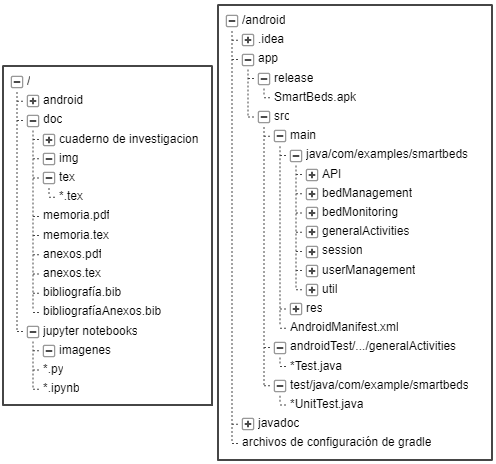
\includegraphics[width=1\textwidth]{../img/directorios.png}
	\caption{Estructura de directorios del repositorio.}
	\label{fig:directorios}
\end{figure}

\section{Manual del programador}

\subsection{Experimentos} 

En el repositorio no se incluye el directorio /data con los ficheros .csv ya que estos datos son propiedad de la empresa proveedora de los datos. Estos datos no son necesarios para poder visualizar los procesos que se han seguido en cada experimento, los distintos métodos que se han empleado y los resultados conseguidos (para ello es necesario tener instalada la herramienta Jupyter Notebook). En todo caso, en el CD proporcionado al tribunal se incluye un enlace a una carpeta en One Drive en el archivo \texttt{data\_link} pero se debe tener en cuenta que estos datos no podrán ser distribuidos ni empleados para usos ajenos a este trabajo. La carpeta \texttt{/data} debe encontrarse en el directorio raíz para poder ejecutar los experimentos. 

En caso de contar con el directorio /data que contiene los datos proporcionados por el proveedor, se recomienda instalar Anaconda, ya que además de incluir Jupyter Notebook, instala por defecto muchas de las bibliotecas que se emplean en los experimentos. Todos los experimentos se han escrito en el lenguaje de programación \textbf{Python 3}. 

\subsection{Aplicación Android}

Para trabajar con el proyecto de Android Studio es necesario tener instalado \textbf{Java JDK 8} y \textbf{Android Studio}. En este caso se ha usado una versión de Android Studio 3.3.2. El resto de dependencias se encuentran indicadas en los ficheros de configuración de gradle, y se añaden automáticamente al construir la aplicación. Concretamente las dependencias de la aplicación se encuentran en el fichero \texttt{/android/app/build.gradle}, y será aquí donde se deberán añadir las dependencias nuevas si son necesarias. En este archivo también se indica la versión mínima de la API de Android que se soporta, en este caso la 23, que corresponde con la versión 6 de Android (\textit{Marshmallow}). Esto supone que la aplicación funcionará en dispositivos con una versión 6 de Android o superior. 

Además, el funcionamiento de esta aplicación depende de los servicios ofrecidos por la API implementada por mi compañero José Luis Garrido Labrador. Los requisitos e instalación de la API del servidor remoto se encuentran documentados en los anexos de su trabajo: \url{https://github.com/jlgarridol/TFG-SmartBeds}.

\section{Compilación, instalación y ejecución del proyecto}

En este apartado se indica cómo importar el proyecto de Android Studio, cómo ejecutar la aplicación y cómo exportar el archivo .apk para la distribución en instalación de la aplicación en un dispositivo Android. 

\subsection{Importar el proyecto}

Una vez instalados Java JDK 8 y Android Studio, para importar el proyecto se deben seguir los siguientes pasos: 

\begin{enumerate}
	\item Acceder al repositorio: \url{https://github.com/aog0036/TFG-SmartBeds}. 
	\item Descargar el contenido del repositorio desde \textbf{Clone or download >~Download ZIP}. 
	\begin{figure}[H]
		\centering
		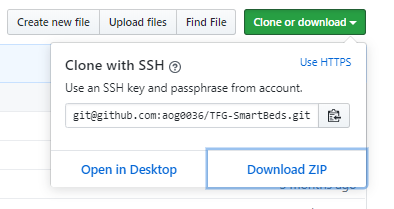
\includegraphics[width=0.5\textwidth]{../img/download.png}
		\caption{Descarga del contenido del repositorio.}
		\label{fig:download}
	\end{figure}
	\item Descomprimir el fichero .zip en la ruta en la que se desee alojar el proyecto. 
	\item Abrir Android Studio. 
	\item En el menú de opciones de Android Studio ir a \textbf{File >~Open} y seleccionar el directorio \textbf{/android}. 
	\begin{figure}[H]
		\centering
		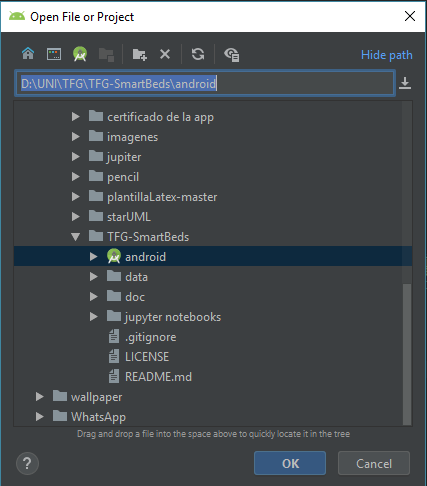
\includegraphics[width=0.5\textwidth]{../img/open.png}
		\caption{Importar proyecto de Android Studio.}
		\label{fig:open}
	\end{figure}
\end{enumerate}

\subsection{Ejecutar la aplicación}

Existen dos formas de ejecutar la aplicación en Android Studio: conectando un dispositivo Android mediante USB o usando un emulador. Para que tu equipo reconozca el dispositivo Android al conectarlo, es necesario que tengas instalados sus \textit{drivers}, por lo demás, es la opción más rápida y cómoda. Por otro lado, si no se dispone de un dispositivo que tenga una versión de Android compatible con la aplicación, puedes crear un nuevo emulador de la siguiente forma: 

\begin{enumerate}
	\item En el menú de opciones ir a \textbf{Run >~Run `app'}. 
	\item En la ventana emergente que se muestra seleccionar la opción \textbf{Create New Virtual Device}. 
	\item Aquí podrás escoger el modelo del dispositivo que quieras emular y la versión de Android a instalar. 
\end{enumerate}

Para ejecutar la aplicación, tanto en un dispositivo conectado al equipo como en el emulador, se siguen los siguientes pasos: 

\begin{enumerate}
	\item En el menú de opciones ir a \textbf{Run >~Run `app'}.
	\item En la ventana emergente seleccionar el dispositivo que quieres usar y pulsar \textbf{OK}. 
\end{enumerate}

\subsection{Exportar apk}

Para exportar el archivo .apk que permite distribuir e instalar la aplicación en un dispositivo Android se siguen los siguientes pasos: 

\begin{enumerate}
	\item En el menú de opciones ir a \textbf{Build >~Build Bundle(s) / APK(s) >~Build APK(s)}. 
	\item El archivo apk generado se encontrará en el directorio \\ \texttt{/android/app/build/outputs/apk/debug}.
\end{enumerate}

Si se desea generar un apk para subirlo a la plataforma Google Play se debe escoger la opción \textbf{Build >~Generate Signed Build / APK...} que crea una apk firmada, asociada a un certificado que es necesario para distribuir la aplicación en Google Play. 

\section{Pruebas del sistema}

Además de las pruebas manuales, se han realizado dos tipos de pruebas del sistema: pruebas unitarias y pruebas de sistema, más concretamente de interfaz de usuario. 

\subsection{Pruebas unitarias} 

Para realizar las pruebas unitarias sobre las clases que no están directamente asociadas con una interfaz de usuario se ha empleado la biblioteca de pruebas unitaria sobre Java \textbf{JUnit}. Las pruebas unitarias comprueban el buen comportamiento de un solo módulo o clase de forma aislada.

Estas pruebas se encuentran en el directorio \\ \texttt{/android/app/src/test/java/com/example/smartbeds}. 

\begin{table}[H]
	\begin{tabularx}{\textwidth}{lX}
		\toprule 
		\textbf{Prueba} & \textbf{Descripción}\\
		\midrule
		BedUnitTest.java & Prueba el funcionamiento de los \textit{getters} y \textit{setters} de la clase Bed. \\
		SessionUnitTest.java & Prueba el comportamiento \textit{singleton} de la clase Session, el funcionamiento de sus \textit{getters} y \textit{setters} y la función \texttt{resetSession}. \\
		\bottomrule
	\end{tabularx}
	\caption{Pruebas unitarias.}
\end{table}

\subsection{Pruebas de interfaz}

Además de las pruebas unitarias, se han realizado una serie de pruebas sobre la interfaz de usuario mediante la herramienta \textbf{Espresso}. Esta herramienta permite grabar las acciones del usuario sobre los elementos de la interfaz de usuario, hacer comprobaciones del contenido tras cada acción y volver a ejecutar la grabación. Este tipo de pruebas resultan más útiles para una aplicación pequeña como esta. 

Para ejecutar las pruebas de interfaz debemos seleccionar el directorio que las contiene en el menú de navegación del proyecto y pulsar \textbf{Run `Tests in `nombre del directorio''}. 

Además, la herramienta Espresso se encuentra completamente integrada en Android Studio, permitiendo generar una nueva prueba de la siguiente forma:

\begin{enumerate}
	\item En el menú de opciones de Android Studio ir a \textbf{Run >~Record Espresso Test}. 
	\item Escoger el dispositivo (real o emulado) sobre el que se desea grabar la prueba y pulsar \textbf{OK}. 
	\item Se abrirá una ventana emergente en la que se irán registrando las acciones. 
	\item Tras cada acción, pulsando en la opción \textbf{Add Assertion} de la ventana emergente se pueden añadir comprobaciones sobre el contenido de la interfaz (por ejemplo, comprobar que cierto elemento está presente o que cierto \textit{TextView} contiene un texto determinado). 
	\item Una vez realizada la grabación al pulsar \textbf{OK} se generará el código correspondiente de la prueba con el nombre que se le indique. 
\end{enumerate} 

Para ejecutar la prueba generada debemos seleccionarla en el menú de navegación del proyecto con click derecho y seleccionar \textbf{Run `nombre del test'}. También podemos ejecutar todas las pruebas seleccionando con click derecho el directorio que las contiene y pulsando \textbf{Run `Tests in `nombre del directorio''}. 

Estas pruebas se encuentran en el directorio \\ \texttt{/android/app/src/androidTest/java/com/example/smartbeds/\\generalActivities}.


\begin{table}[H]
	\begin{tabularx}{\textwidth}{lX}
		\toprule 
		\textbf{Prueba} & \textbf{Descripción}\\
		\midrule
		loginTest.java & Prueba el correcto funcionamiento de la pantalla de inicio de sesión. \\
		changePassTest.java & Prueba el correcto funcionamiento de la pantalla de cambio de contraseña. \\
		addDeleteUserTest.java & Prueba las funciones añadir y eliminar usuario, comprobando que un usuario eliminado no puede acceder al sistema. \\
		asignUserBedTest.java & Prueba que la asignación de una cama a un usuario funciona correctamente. \\
		navigationTest.java & Prueba el correcto funcionamiento del menú de navegación y todas sus opciones. \\
		\bottomrule
	\end{tabularx}
	\caption{Pruebas de interfaz.}
\end{table}
